\documentclass[]{beamer}

%\userpackage[latin1]{inputenc}
\usepackage[utf8]{inputenc}
\usepackage[T1]{fontenc}
\usepackage[french]{babel}
\usepackage{xcolor,colortbl,array,graphicx}
\usepackage{times}
\usepackage{amsthm,amsmath,amsfonts,amssymb,amstext}
\usepackage{lipsum}
\usepackage{hyperref,url}

\title[Arduino]{Les bases de l'automatisme avec l'Arduino}
% ----------------------
\author[Michel Nassalang]{}
% ----------------------
\institute[IPSL]{
Lycée Amadou Sow Ndiaye}
% ----------------------
\date[]{Arduino}

% ----------------------
\mode <presentation> {
\usetheme{Montpellier}
%{Bergen}{PaloAlto}{Berkeley}{Boadilla}{Pittsburgh}{Rochester}
%{Antibes}{Montpellier}{JuanLesPins}{Berkeley}
\usecolortheme{whale}
%{whale} {orchid}{owl}{albatross}{beaver}
\usefonttheme{professionalfonts}
%{professionalfonts} {serif}{structurebold}
%{structureitalicserif}{structuresmallcapsserif}
\useoutertheme{infolines}
%{infolines} {miniframes}{shadow}{sidebar}
%{smoothbars}{smoothtree}{split}{tree}
\useinnertheme{rectangles}
%{circles}{rounded}{rectangles}{inmargin}
\setbeamercovered{transparent=50}
}
\AtBeginSection[]
{
\begin{frame}
<beamer>
\frametitle{\sc Sommaire}
\tableofcontents[currentsection,currentsubsection]

\end{frame}
}

\begin{document}
	\begin{frame}
		\titlepage		
		\begin{figure}
			\begin{center}
				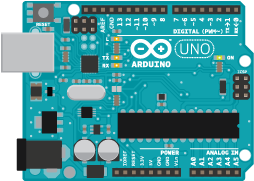
\includegraphics[scale=0.5]{arduino.png}
			\end{center}
		\end{figure}
	\end{frame}
	\section{Arduino}
	\subsection{Définition}
	\begin{frame}
	{Définition de la Carte Arduino}
	\begin{itemize}
	\item \textbf{Carte Arduino}
	 \\Une carte Arduino est une petite carte électronique 				équipée d'un micro-controlleur. La carte est une interface  				programmable quipermet de réaliser beaucoup d'actions avec 				l'appui des actionneurs et des capteurs. La carte se relie à un 		ordinateur par un câble USB.
	\item \textbf{Mitrocontrolleur}
	  \\Un micro-controlleur est un système qui ressemble à un 		ordinateur: il a une mémoire, un processeur, des interfaces 				avec le monde extérieur.
	\end{itemize}
	\end{frame}
	\subsection{Types d'Arduino}
	\begin{frame}
	{Types de cartes}
	Nous avons plusieurs types de cartes Arduino à savoir :
	\begin{figure}
	\begin{center}
	 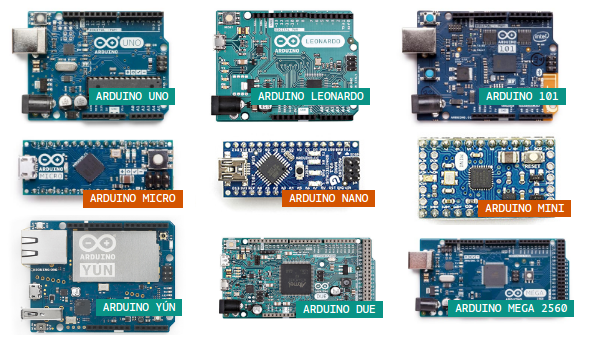
\includegraphics[scale=0.5]{types-arduino.png}
	\end{center}
	\end{figure}
	\end{frame}
	\section{Matériels nécessaires pour l'Arduino}
	\subsection{Capteurs}
	\begin{frame}
	{Capteurs pour Carte Arduino}
	 Les capteurs pour les cartes Arduino sont multiples.
	Nous avons l'ultrason qui permet de détecter des objets environnants, les capteurs de lumière, les thermomètres infrarouges, les capteurs d'humidité des sols, les capteurs de son, les capteurs de flamme, les capteurs d'altitude et de pression, les détecteurs d'obstacles, les capteurs de mouvement ...
	\end{frame}
	\subsection{Câblage}
	\begin{frame}
	{Les connections}
	\begin{itemize}
		\item \textbf{Alimentation} \\
		Les cartes Arduino sont souvent alimentées par des cables délivrant une tension avec une intensité atteignant au maximum 12V.
		\item \textbf{Jumpers} \\
		Les jumpers sont les petites cables de test à utiliser pour établir les connections entre une carte Arduino et les capteurs et les actionneurs.
	\end{itemize}
	\end{frame}
	\begin{frame}
	{kit Arduino}
	 Le kit est composé de tous les matériels nécessaires pour réaliser des projets et des faire des tests et des réalisations électroniques.
	 \begin{figure}
	 	\begin{center}
	 		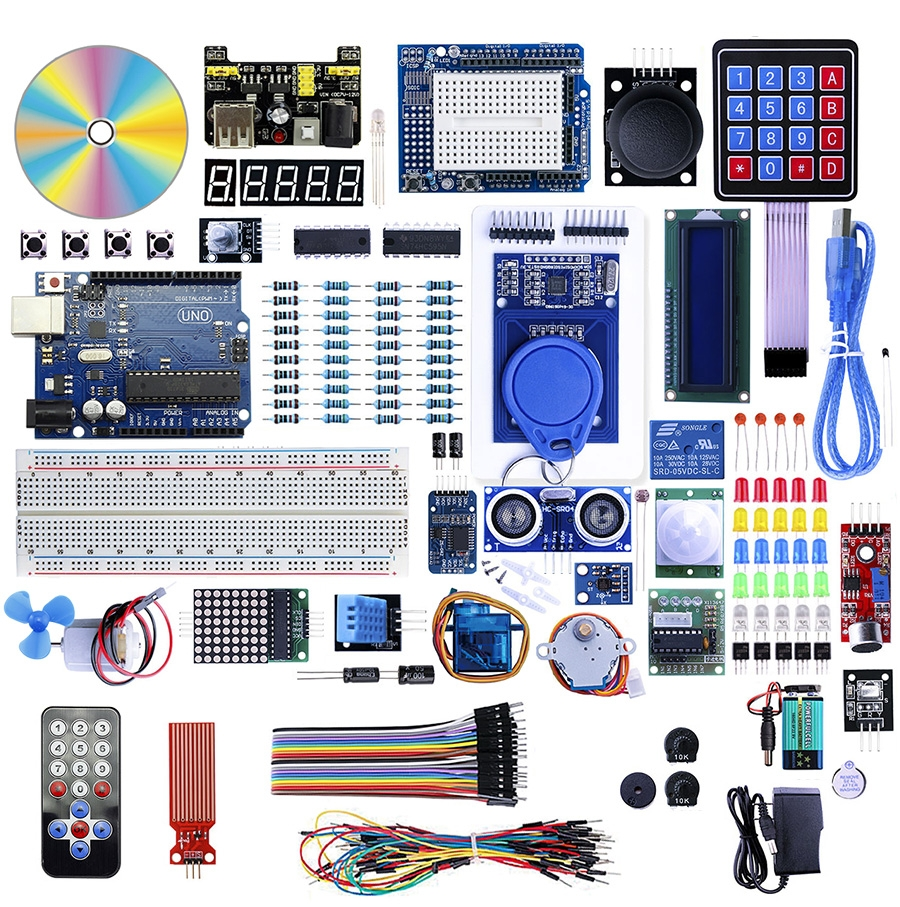
\includegraphics[scale=0.25]{modules_for_arduino.jpg}
	 	\end{center}
	 \end{figure}
	\end{frame}
	\section{Projets et réalisation avec Arduino}
	\subsection{Tests et utilisations des matériels du kit arduino}
	\begin{frame}
		{Tests}
			Nous pouvons réaliser des tests avec les actionneurs et les 
			capteurs. Les exemples sont les suivantes sur les figures:
			\begin{figure}
				\begin{center}
					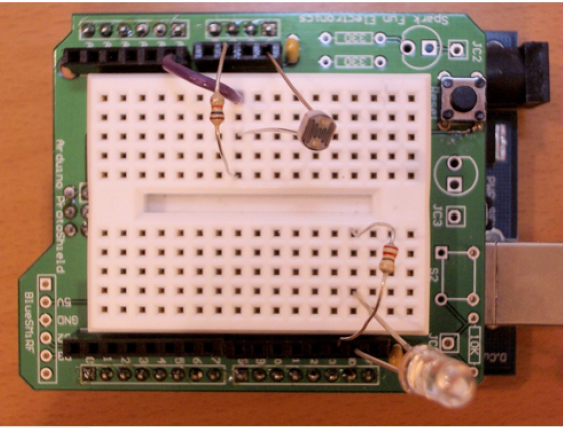
\includegraphics[scale=0.5]{test1.png}
				\end{center}
			\end{figure}
			\begin{figure}
				\begin{center}
					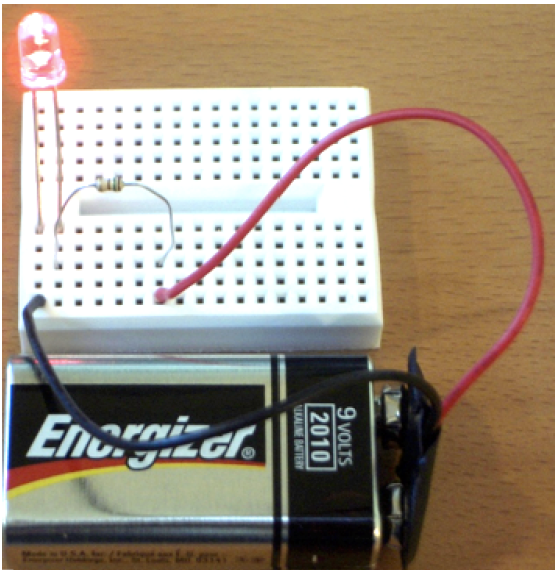
\includegraphics[scale=0.5]{test2.png}
				\end{center}
			\end{figure}
	\end{frame}
	\begin{frame}
	{Tests}
			\begin{figure}
				\begin{center}
					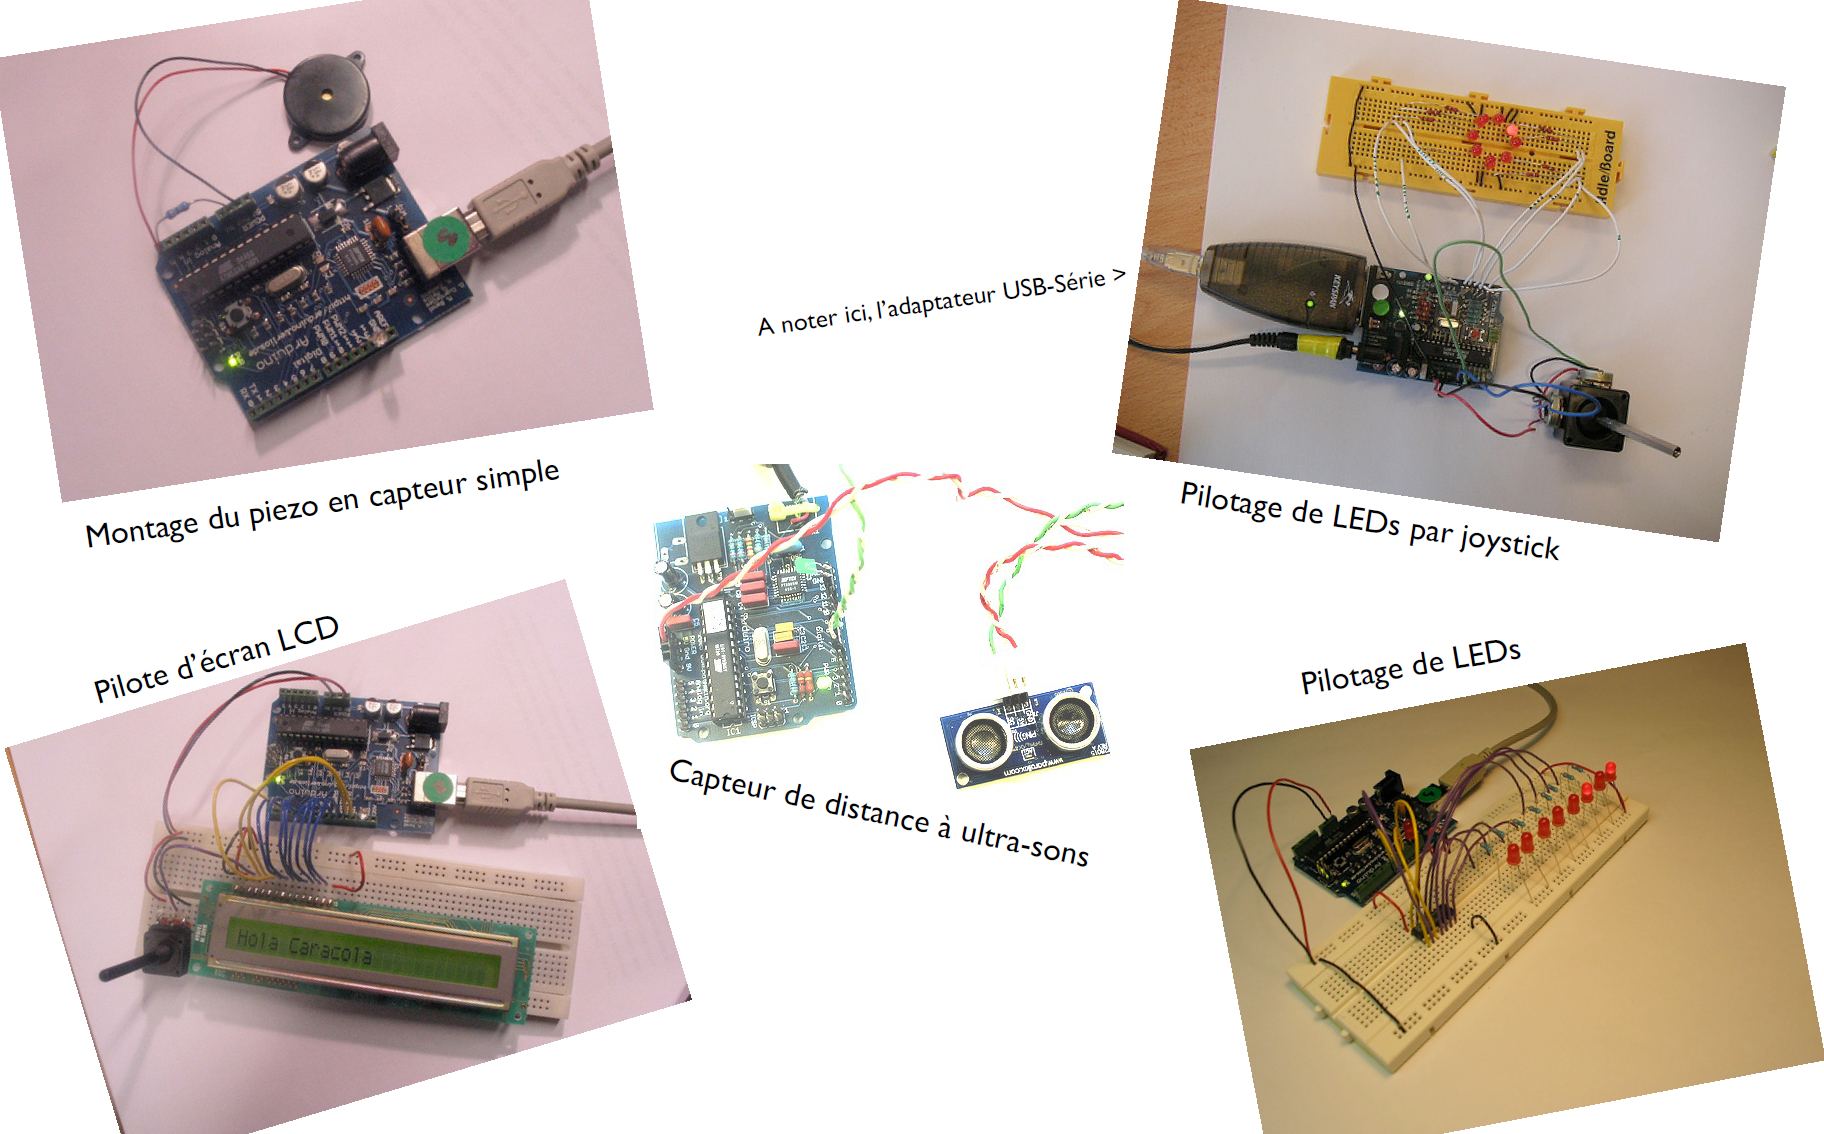
\includegraphics[scale=0.5]{test3.png}
				\end{center}
			\end{figure}
	\end{frame}
	\subsection{Projets réalisables}
	\begin{frame}
		{Projets réalisables}
		Nous pouvons réaliser des projets très avancés avec l'Arduino.
		Les illustrations en sont les suivantes:
		
			\begin{figure}
				\begin{center}
					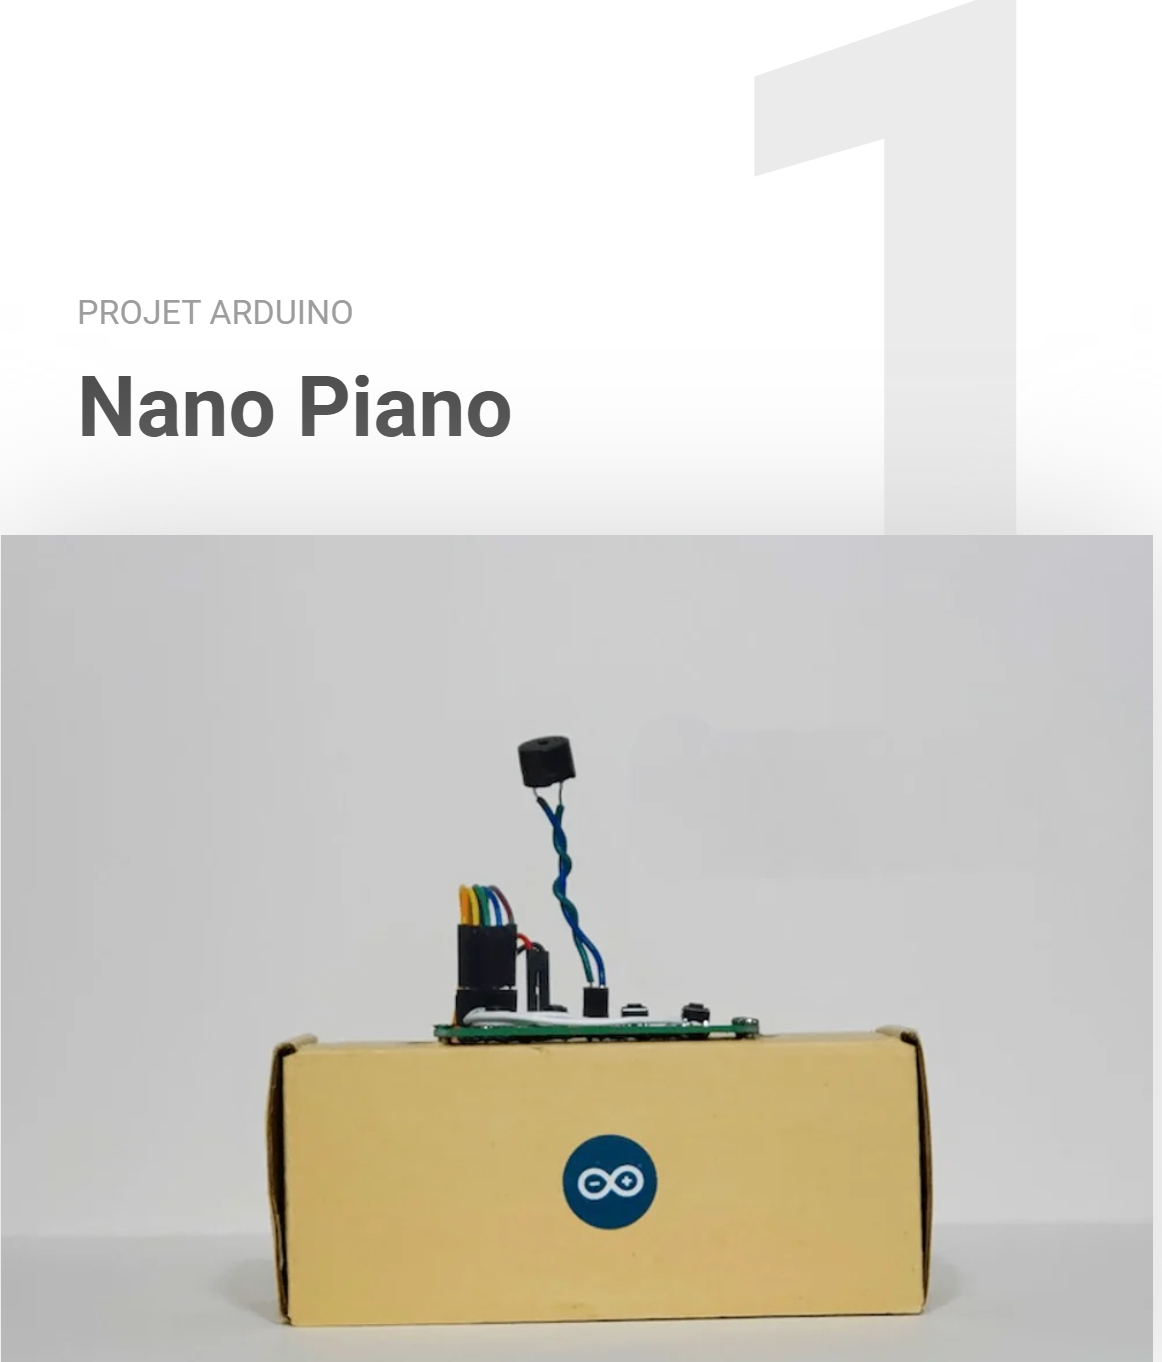
\includegraphics[scale=0.4]{piano_arduino.png}
				\end{center}
			\end{figure}
	\end{frame}
	\begin{frame}
	{Projets réalisables}
			\begin{figure}
				\begin{center}
					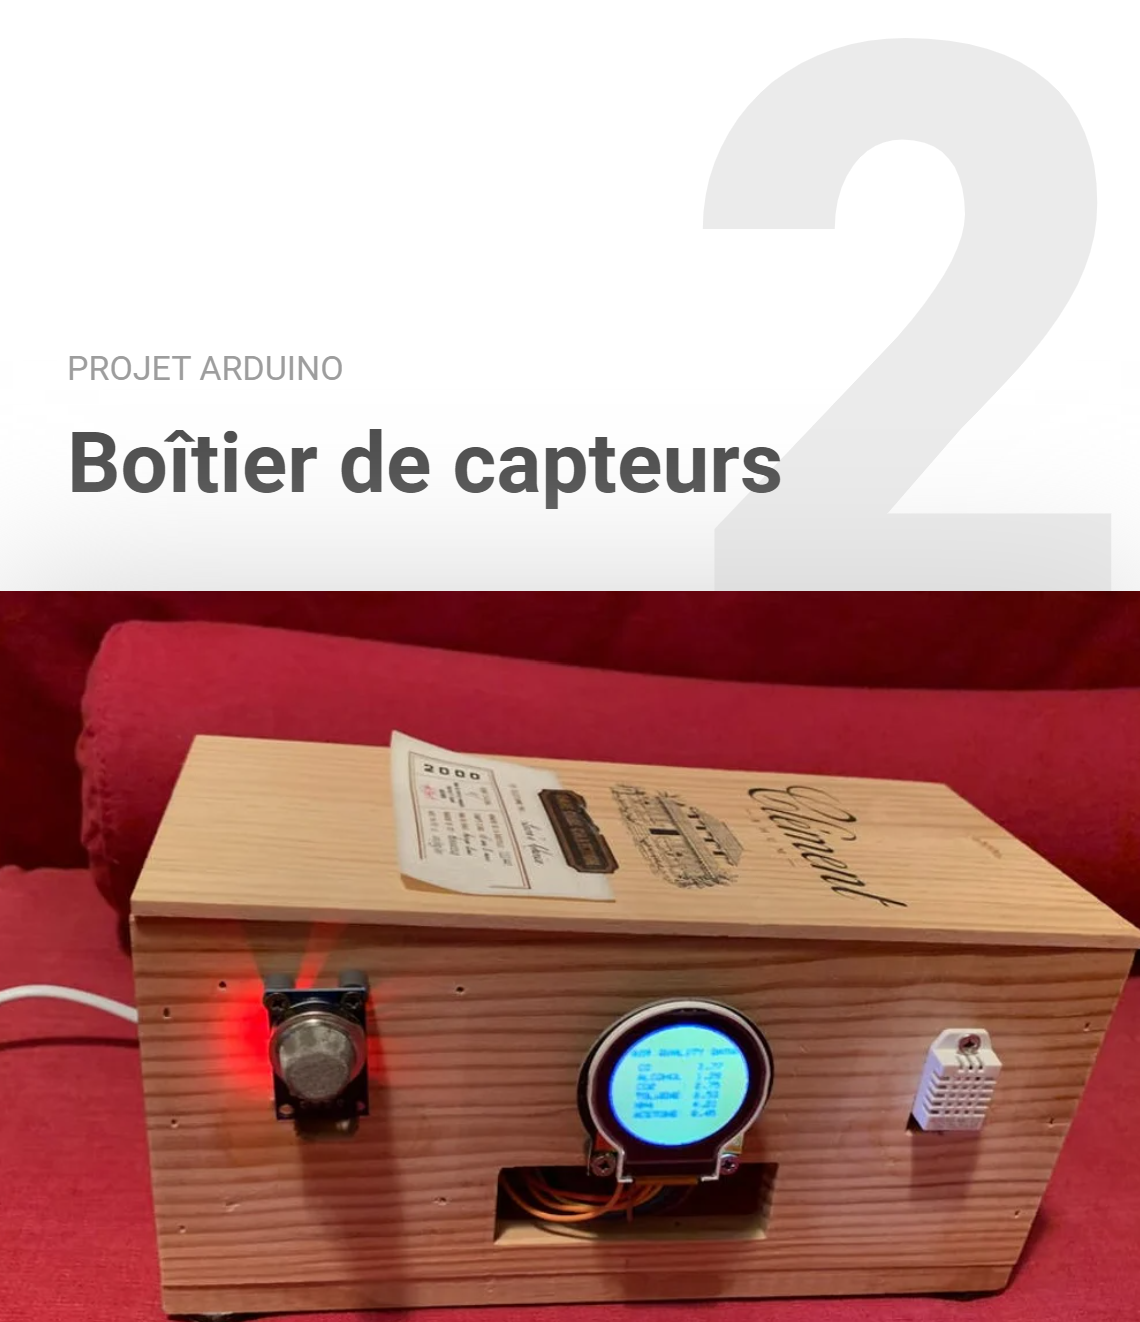
\includegraphics[scale=0.4]{boitier_capteur.png}
				\end{center}
			\end{figure}
	\end{frame}
	\begin{frame}
	{Projets réalisables}
			\begin{figure}
				\begin{center}
					\includegraphics[scale=0.4]{machine_dés.png}
				\end{center}
			\end{figure}
	\end{frame}
	\begin{frame}
	{Projets réalisables}
			\begin{figure}
				\begin{center}
					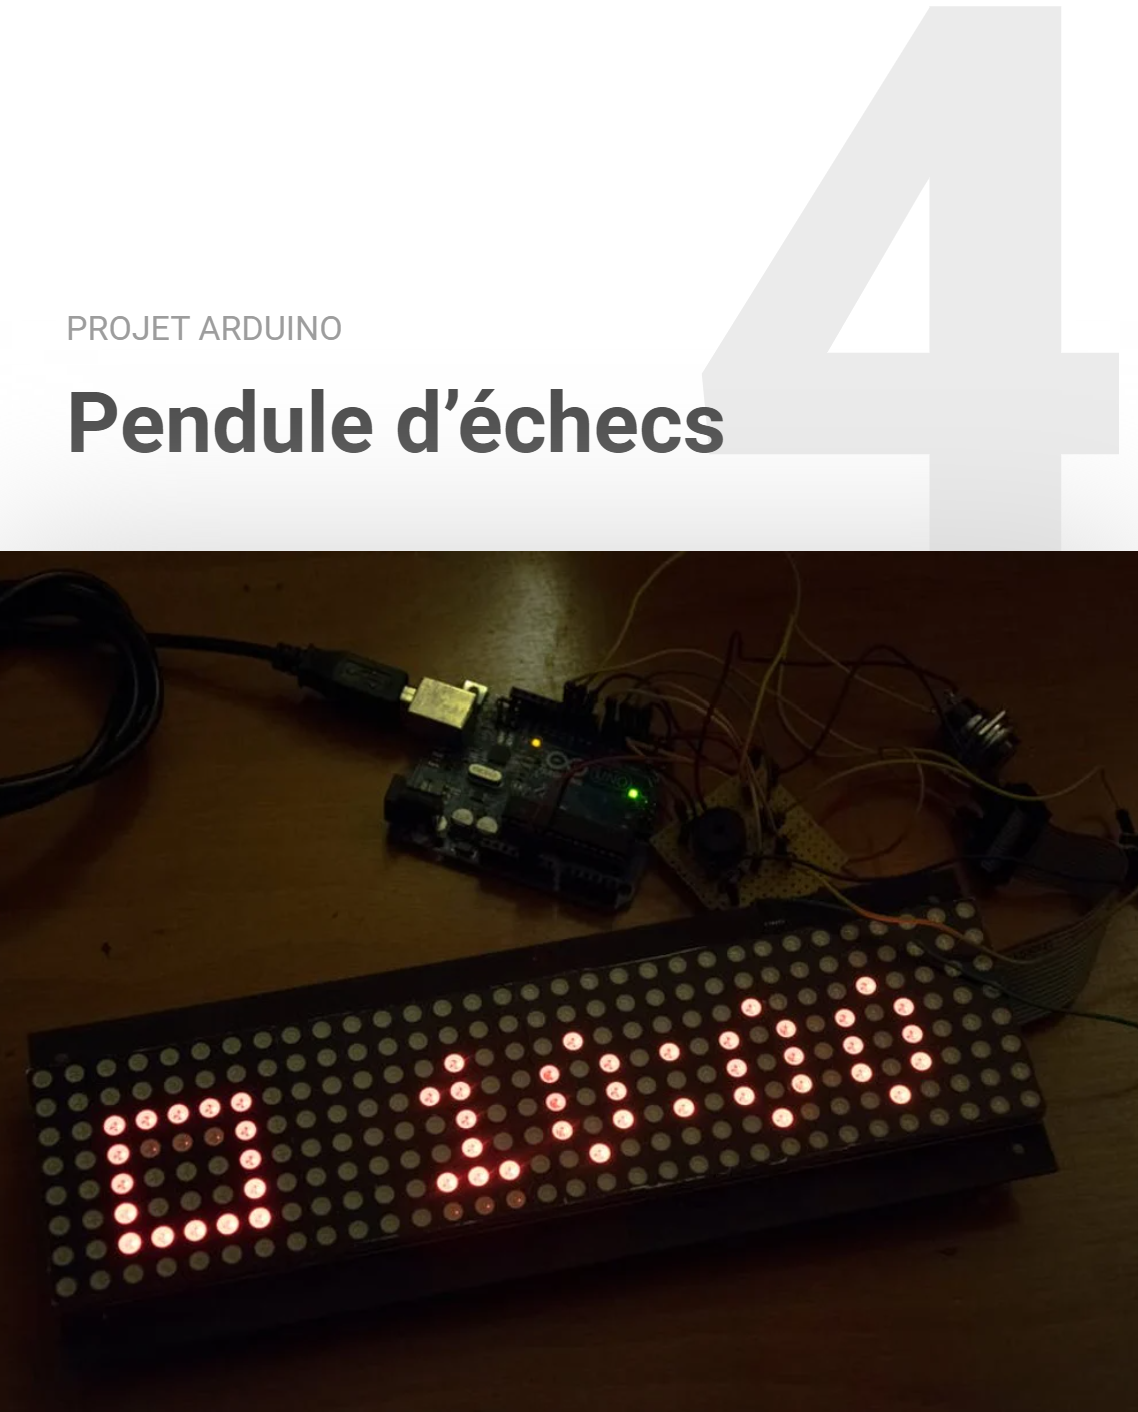
\includegraphics[scale=0.4]{pendule_echec.png}
				\end{center}
			\end{figure}
	\end{frame}
	\begin{frame}
	{Projets réalisables}
			\begin{figure}
				\begin{center}
					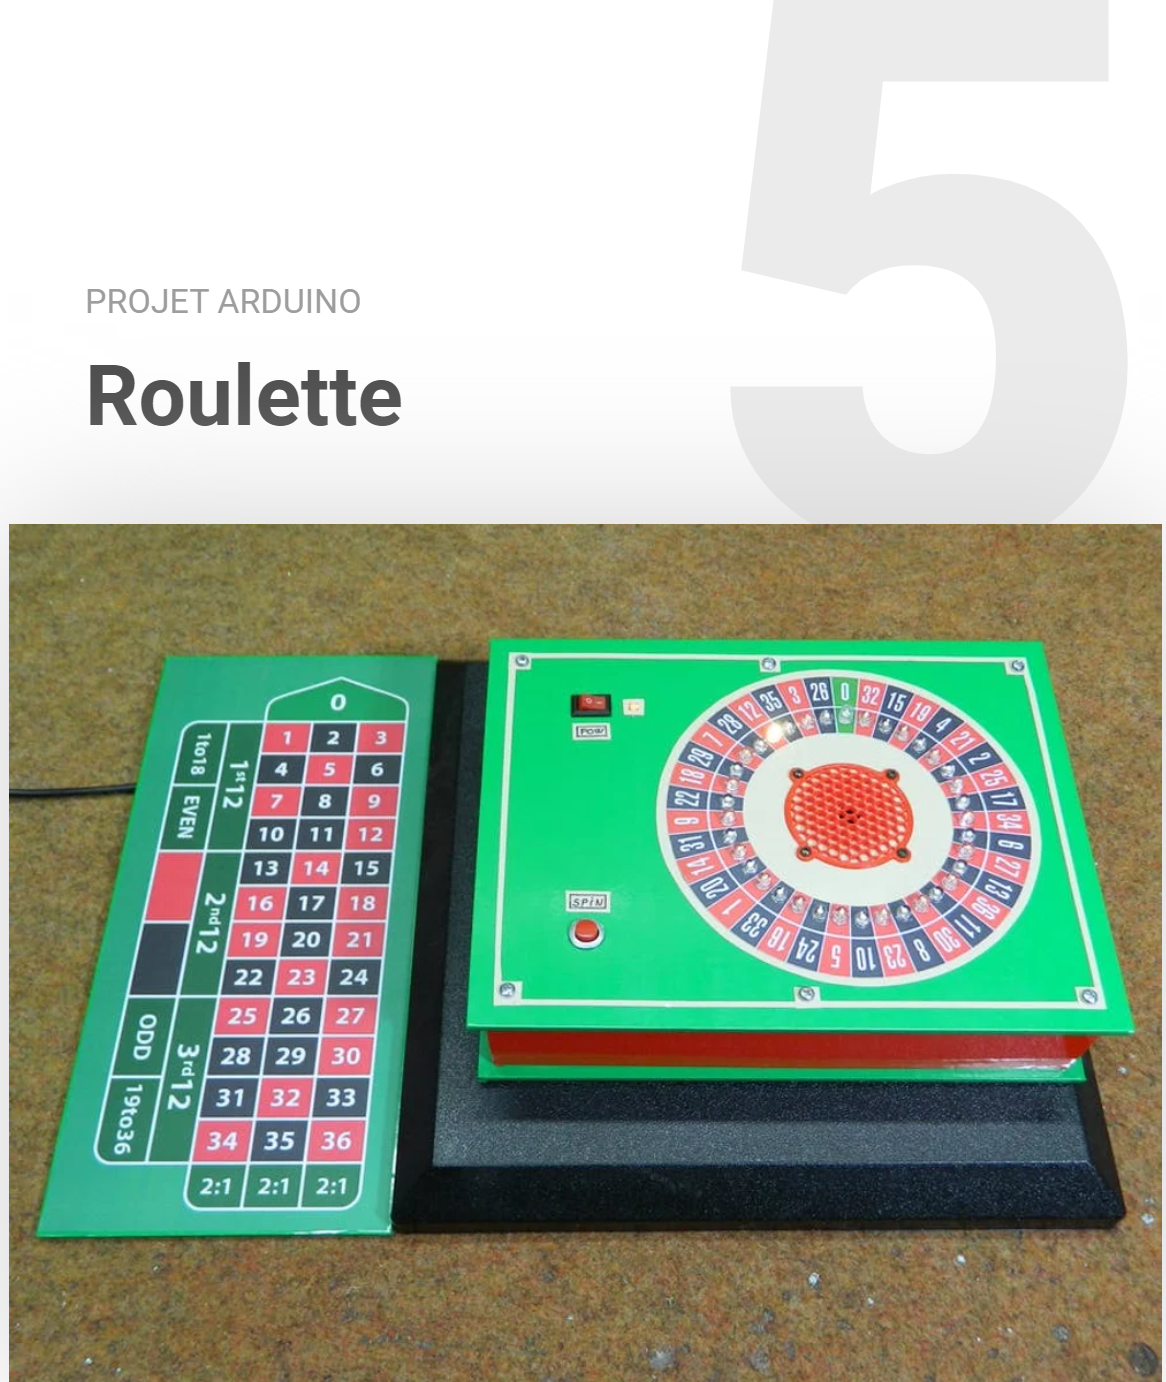
\includegraphics[scale=0.4]{roulette.png}
				\end{center}
			\end{figure}
	\end{frame}
	\begin{frame}
	{Projets réalisables}
			\begin{figure}
				\begin{center}
					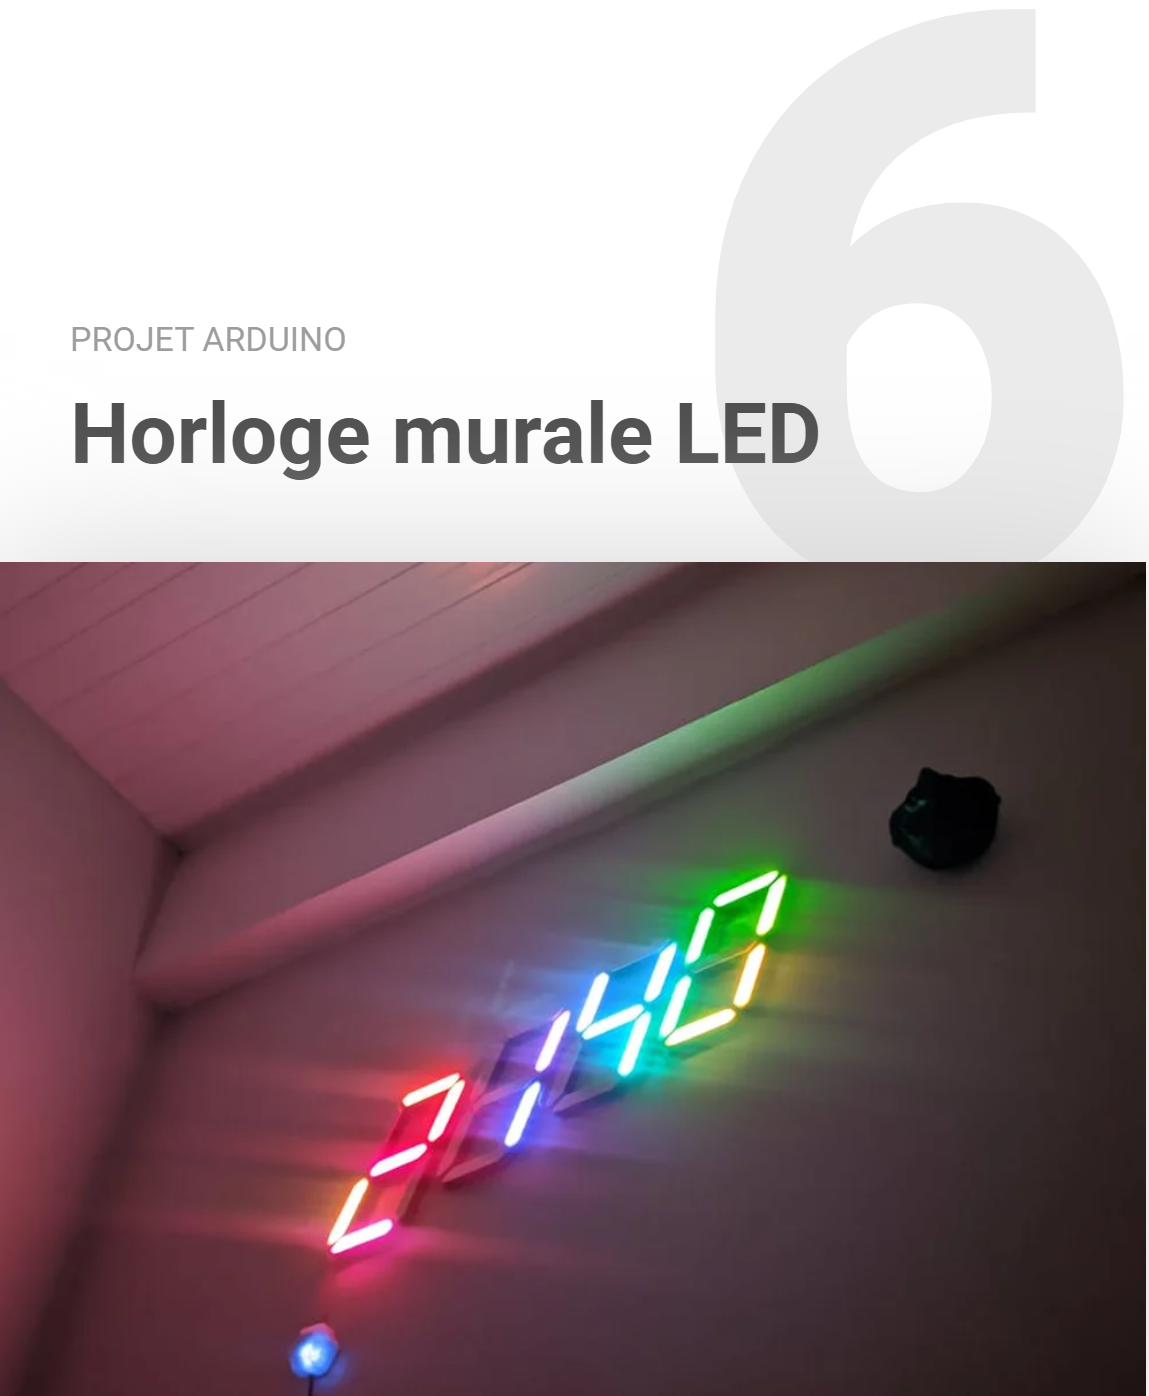
\includegraphics[scale=0.4]{horloge.png}
				\end{center}
			\end{figure}
	\end{frame}
	\begin{frame}
	{Projets réalisables}
			\begin{figure}
				\begin{center}
					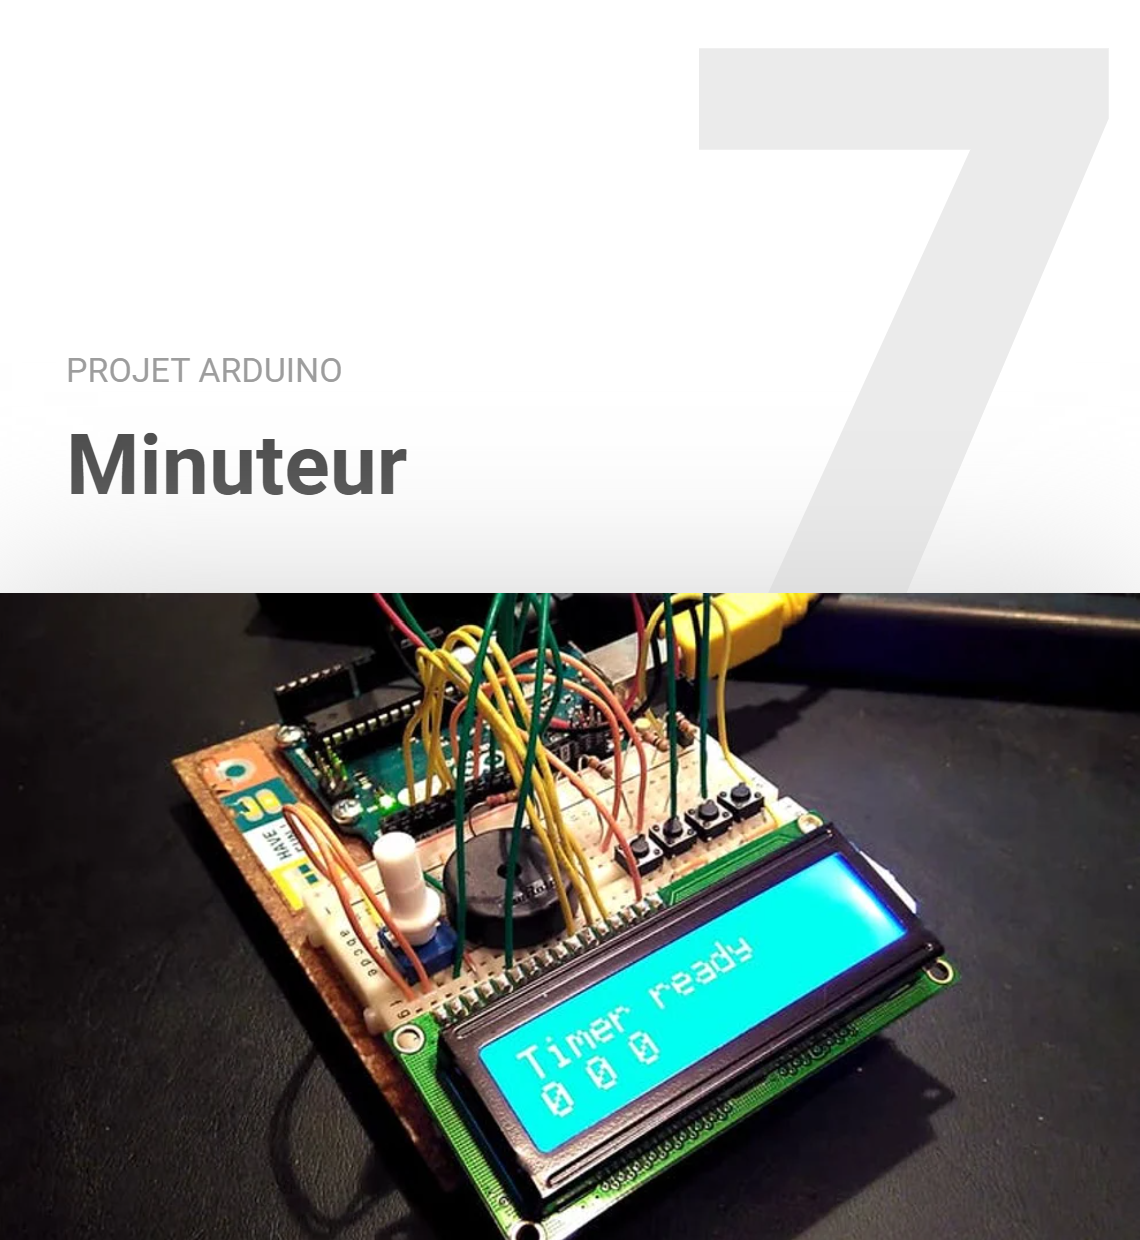
\includegraphics[scale=0.4]{muniteur.png}
				\end{center}
			\end{figure}
	\end{frame}
	\begin{frame}
	{Projets réalisables}
			\begin{figure}
				\begin{center}
					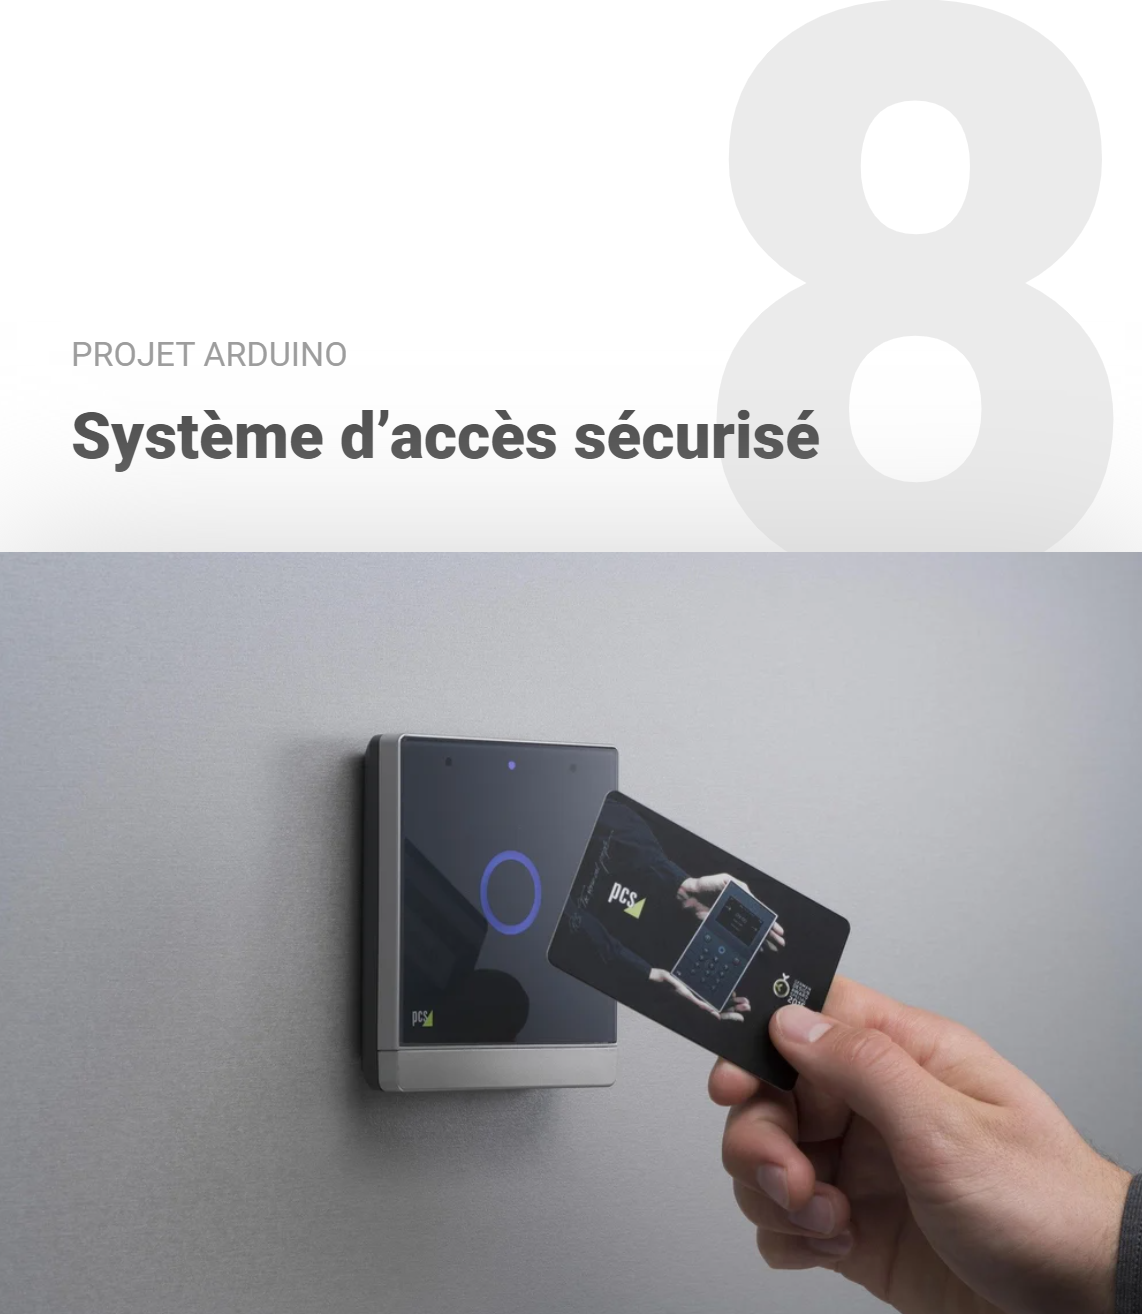
\includegraphics[scale=0.4]{securite.png}
				\end{center}
			\end{figure}
	\end{frame}
	\begin{frame}
	{Projets réalisables}
			\begin{figure}
				\begin{center}
					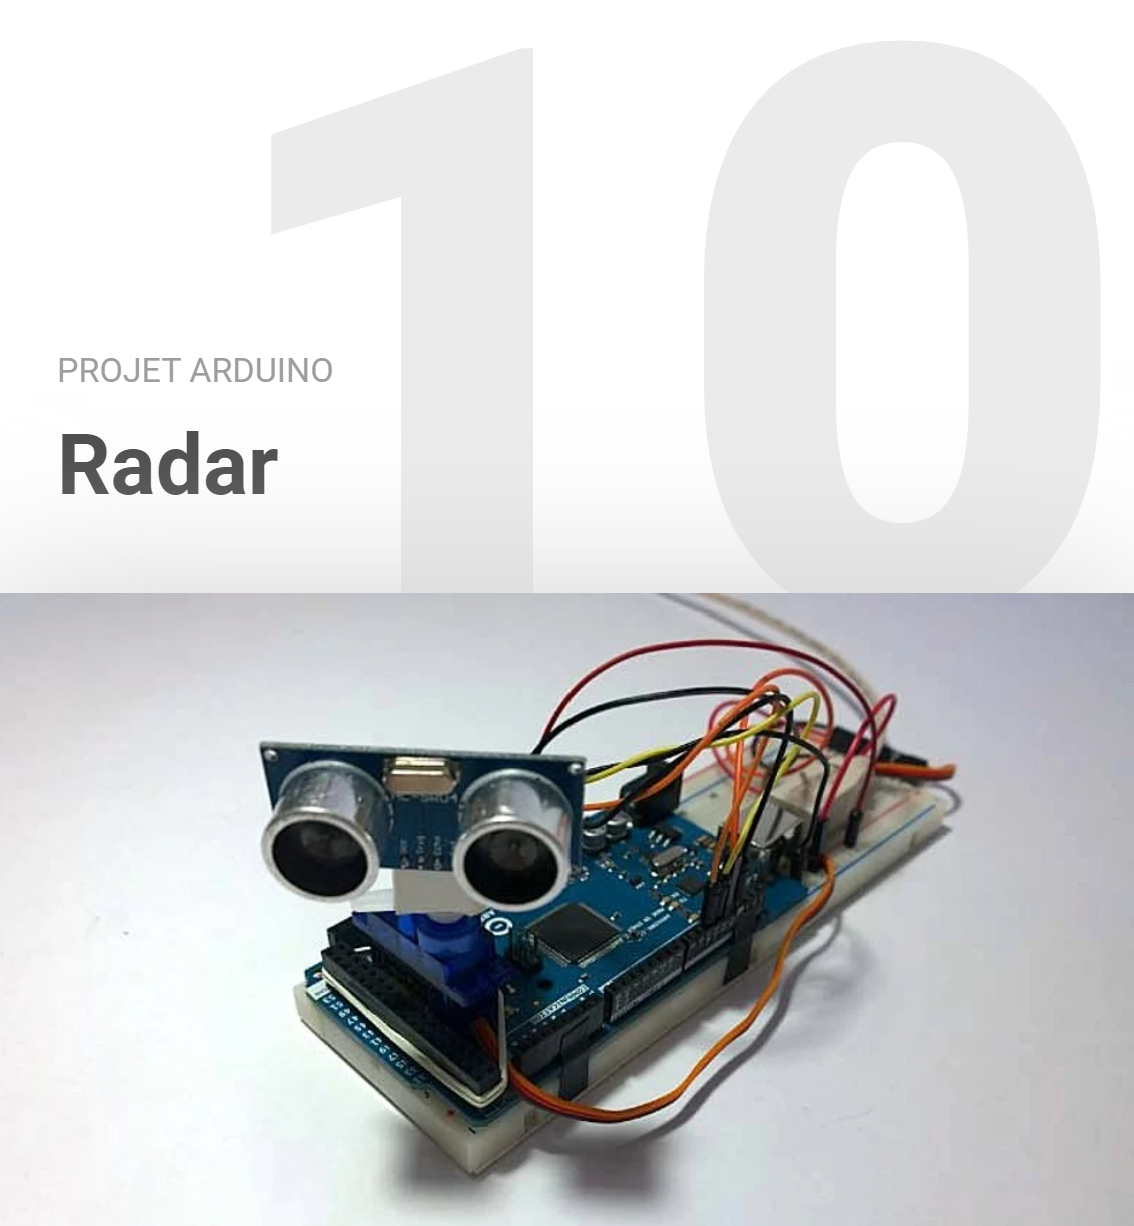
\includegraphics[scale=0.4]{radar.png}
				\end{center}
			\end{figure}
	\end{frame}
	\begin{frame}
	{Projets réalisables}
			\begin{figure}
				\begin{center}
					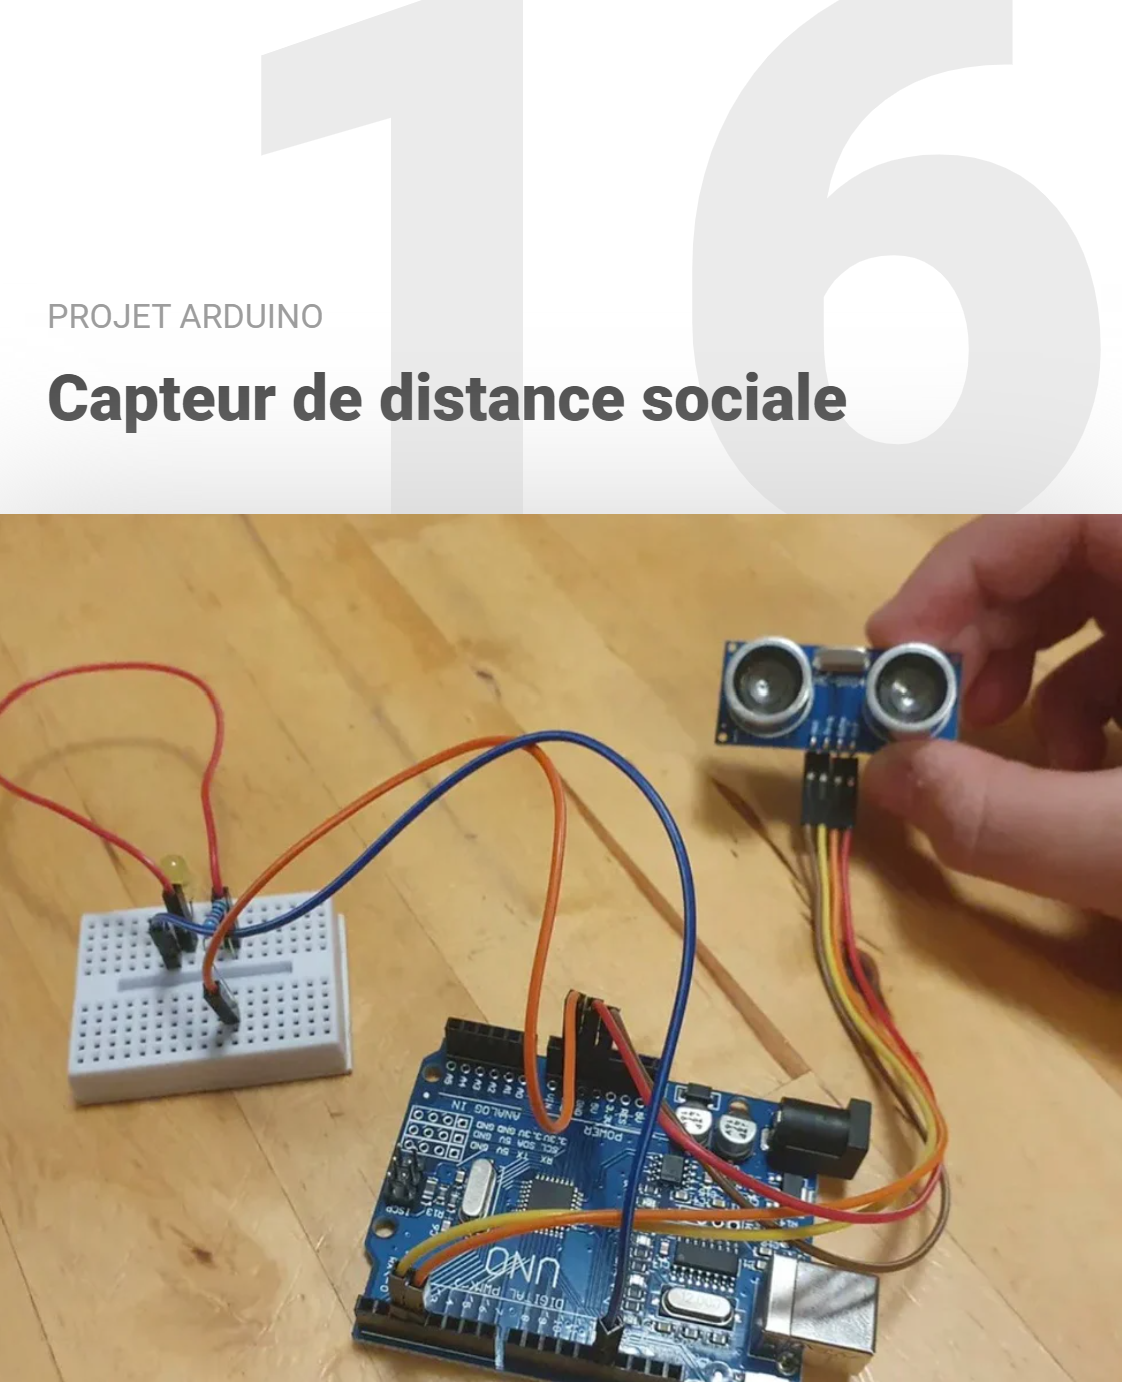
\includegraphics[scale=0.4]{distance.png}
				\end{center}
			\end{figure}
	\end{frame}
	\begin{frame}
	{Projets réalisables}
			\begin{figure}
				\begin{center}
					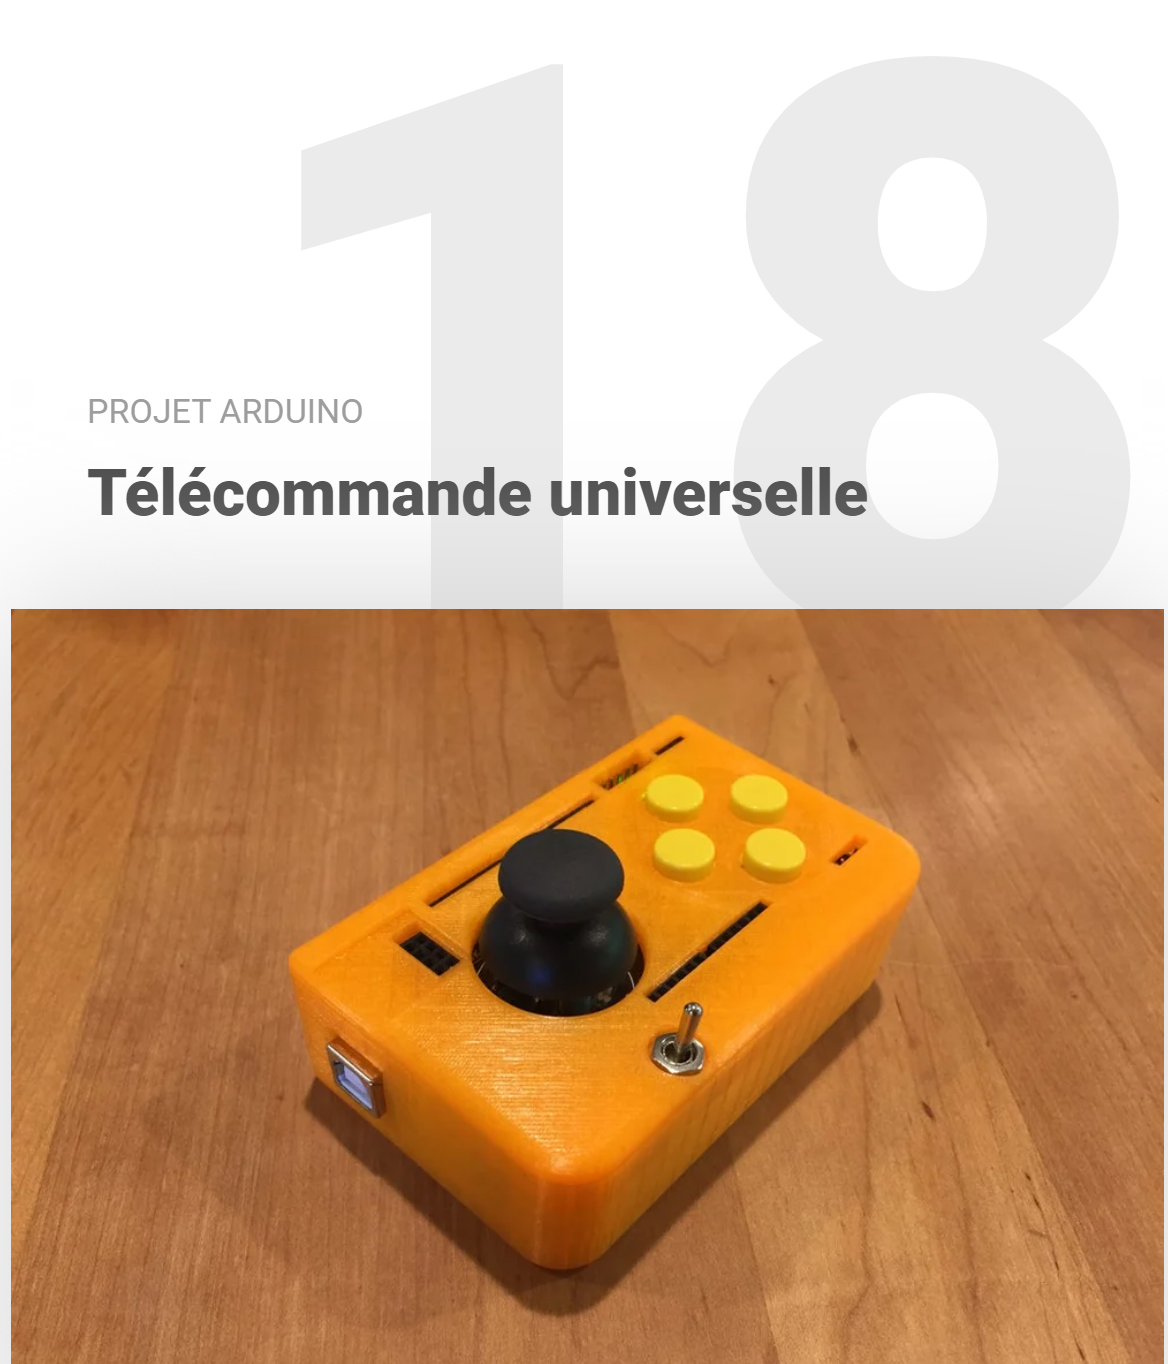
\includegraphics[scale=0.4]{telecommande.png}
				\end{center}
			\end{figure}
	\end{frame}
	\begin{frame}
	{Projets réalisables}
			\begin{figure}
				\begin{center}
					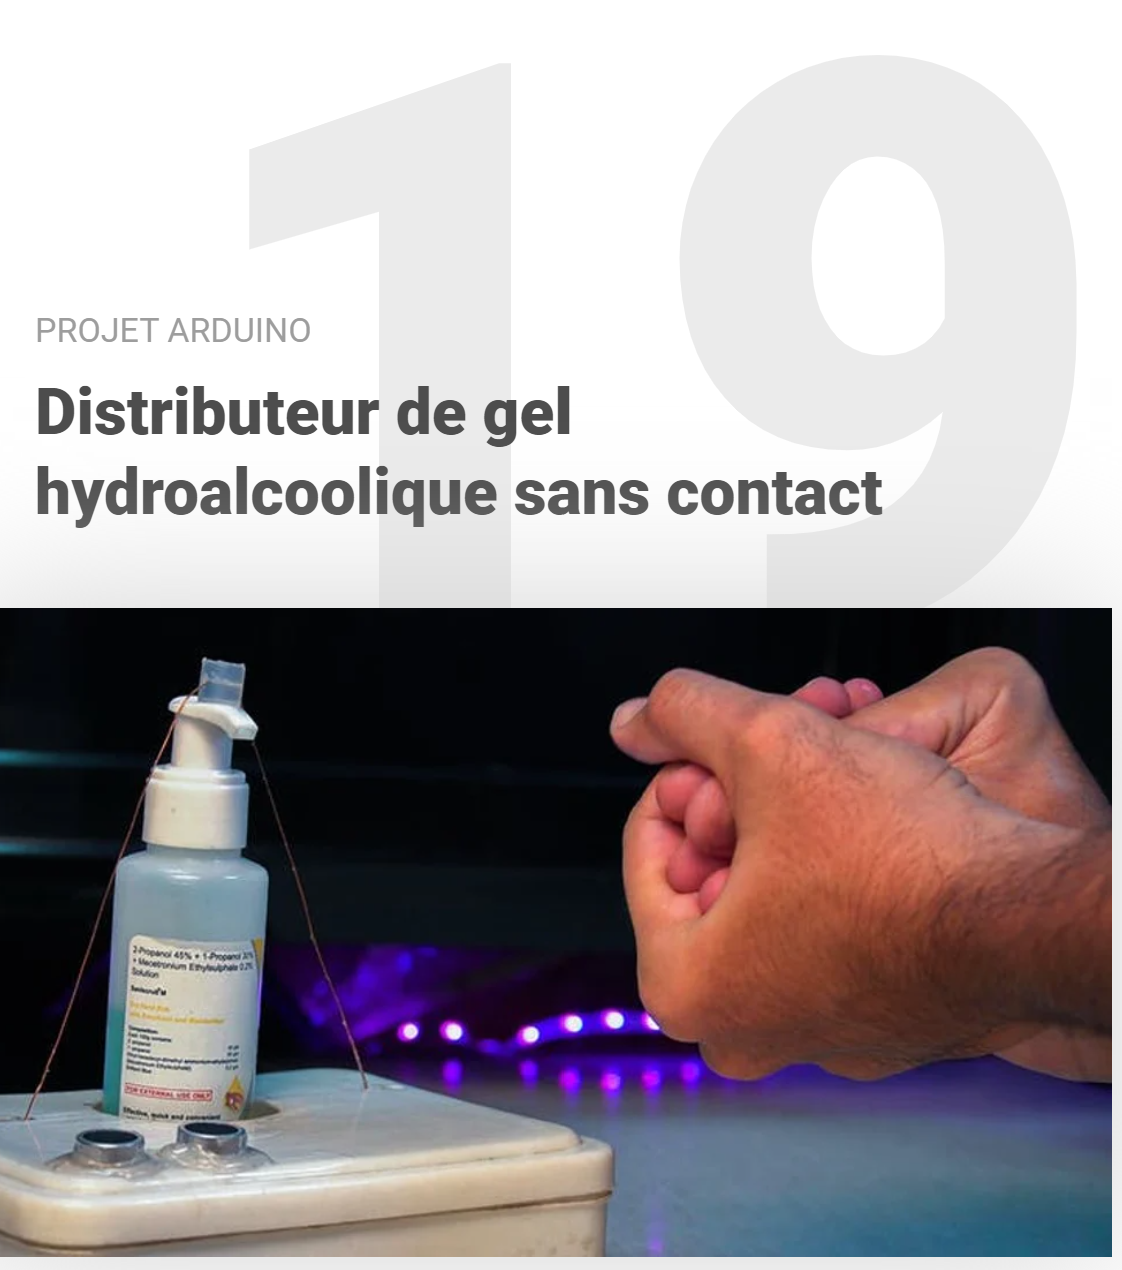
\includegraphics[scale=0.4]{distributeur_gel.png}
				\end{center}
			\end{figure}
	\end{frame}
\end{document}



